% !TEX root = ../STP_journal.tex
\subsection{Numerical Simulations \label{sec:sim_dstb}}
We demonstrate our proposed methods for accounting for disturbances and incomplete information using a four-vehicle example. Each vehicle has the simple kinematics model in \eqref{eqn:NumSimpleDyn} but with disturbances added to the evolution of each state:
\begin{equation}
\label{eq:dyn_i}
\begin{aligned}
\dot{\pos}_{x,i} &= v_i \cos \theta_i + d_{x,i} \\
\dot{\pos}_{y,i} &= v_i \sin \theta_i + d_{y,i}\\
\dot{\theta}_i &= \omega_i + d_{\theta,i}, \\
\underline{v} & \le v_i \le \bar{v}, |\omega_i| \le \bar{\omega},\\
\|(d_{x,i}, & d_{y,i}) \|_2 \le d_{r}, |d_{\theta,i}| \le \bar{d_{\theta}}
\end{aligned}
\end{equation}

\noindent where $d = (d_{x,i}, d_{y,i}, d_{\theta,i})$ represents $\veh_i$'s disturbances in the three states. The control of $\veh_i$ is $u_i = (v_i, \omega_i)$, where $v_i$ is the speed of $\veh_i$ and $\omega_i$ is the turn rate; both controls have a lower and upper bound. For illustration purposes, we choose $\underline{v} = 0.5, \bar{v} = 1, \bar\omega = 1$; however, our method can easily handle the case in which these inputs differ across vehicles. The disturbance bounds are chosen as $d_r = 0.1, \bar{d_{\theta}} = 0.2$, which correspond to a 10\% uncertainty in the dynamics. %The optimal control for vehicle $i$ can be obtained by optimizing the associated Hamiltonian, $H_i(t, D_{\bm{x}_i} V_i(\bm{x}_i,t), V_i(\bm{x}_i,t))$, and is given by:

%\begin{equation}
%\omega_i(t) = -\bar{\omega}_i \frac{D_{\theta_i}V_i(\bm{x}_i,t)}{\left| D_{\theta_i}V_i(\bm{x}_i,t) \right|},
%\end{equation}
%
%\begin{equation}
%v_i(t) =
%\left \{ 
%\begin{array}{ll}
%\underline{v} & \mbox{ if } D_{x_i}V_i(\bm{x}_i,t) \cos \theta_i + D_{y_i}V_i(\bm{x}_i,t) \sin \theta_i \geq 0 \\
%\bar{v} & \mbox{ otherwise } 
%\end{array}
%\right.
%\end{equation}

\begin{figure}[H]
  \centering
  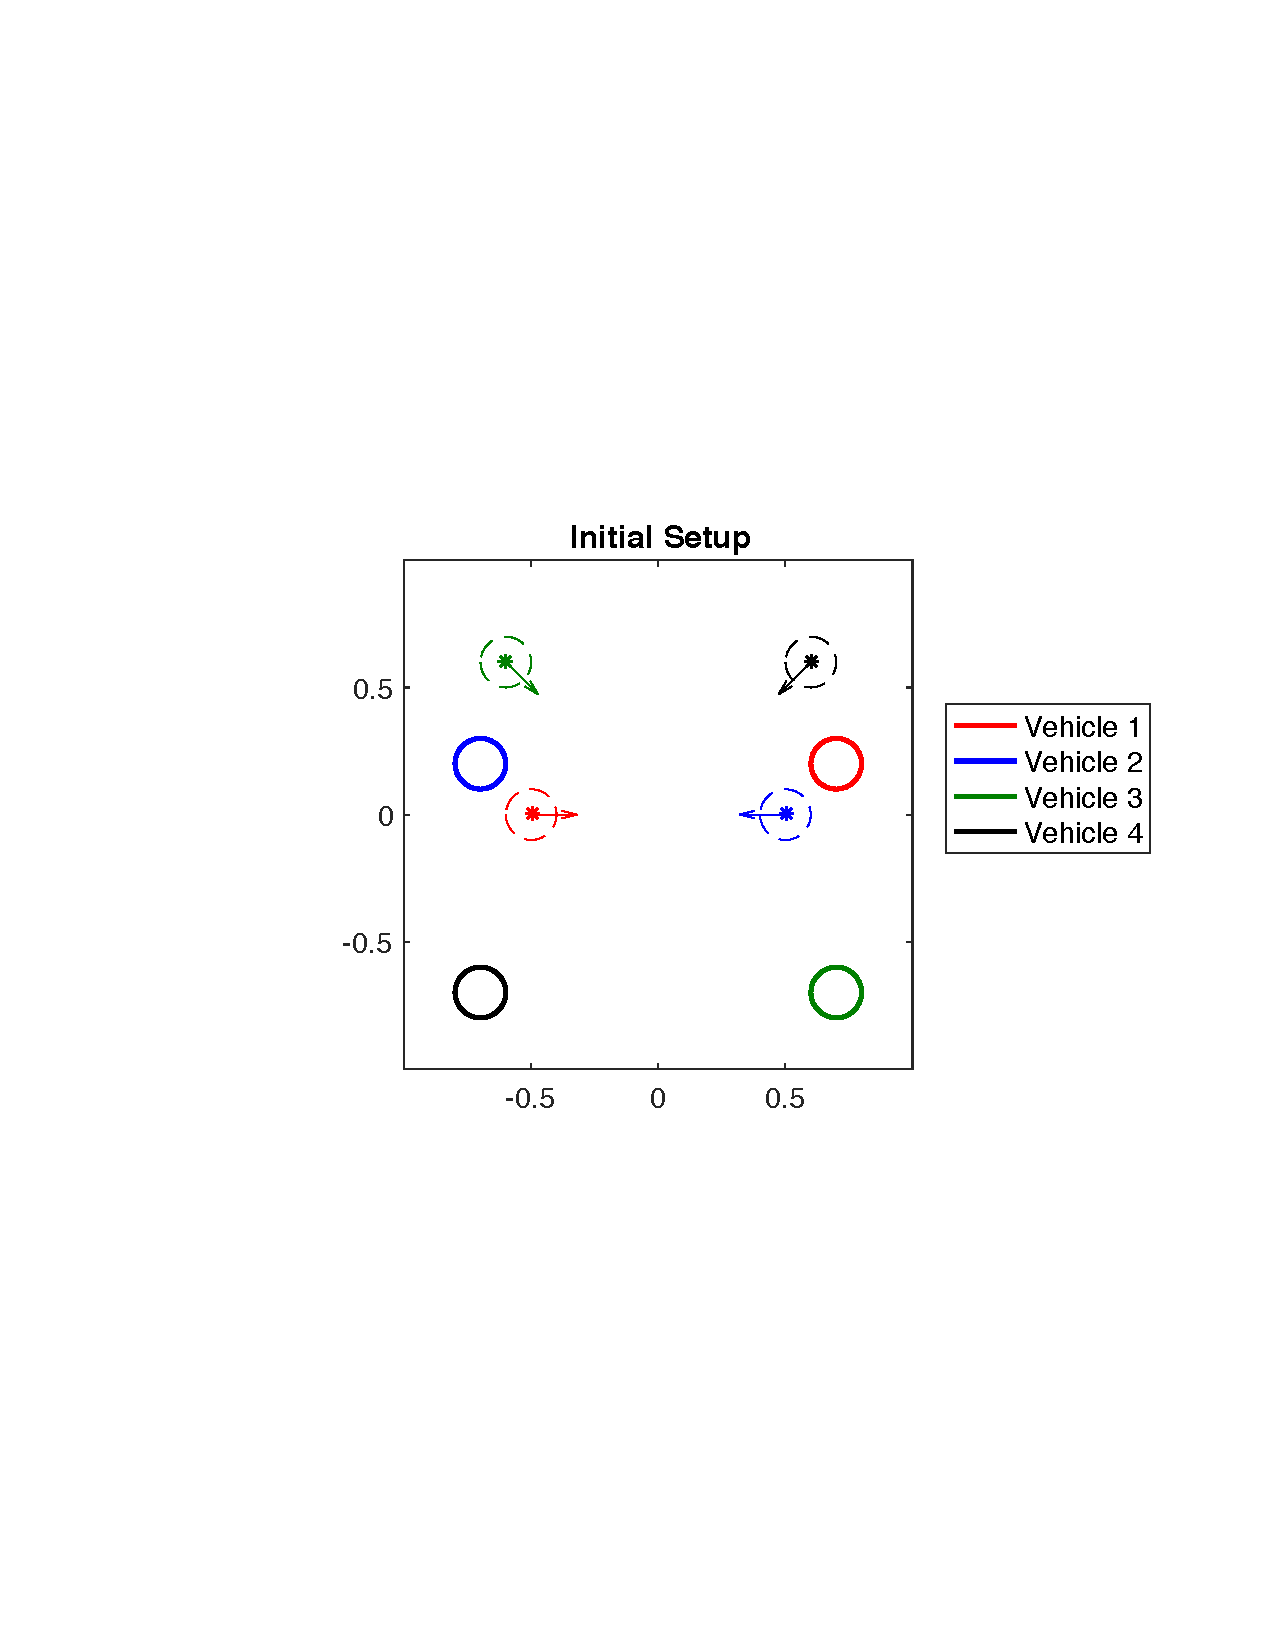
\includegraphics[width=0.6\columnwidth]{fig/init_setup}
  \caption{Initial configuration of the four-vehicle example in the presence of disturbances.}
  \label{fig:init_setup_dstb}
\end{figure}

For this example, we have chosen scheduled times of arrival $\sta_i = 0~\forall i$ for simplicity. Each vehicle aims to get to a target set of radius $r=0.1$. The vehicles' target centers $c_i$ and initial conditions $\state_i^0$ are given by \eqref{eqn:NumIC}. These parameters are the same as the example in Section \ref{sec:basic_results}, except that the $\sta_i$ values are the same for all vehicles, and that there are no static obstacles. The problem setup for this example is shown in Fig. \ref{fig:init_setup_dstb}.

With the above parameters, we obtain $\ldt_i, i=1,2,3,4$. Note that even though $\sta_i$ is assumed to be same for all vehicles in this example for simplicity, our method can easily handle the case in which $\sta_i$ is different for each vehicle as we have already shown in Section \ref{sec:basic_results}.

For each proposed method of computing induced obstacles, we show the vehicles' entire trajectories (colored dotted lines), and overlay their positions (colored asterisks) and headings (arrows) at a point in time in which they are in a relatively dense configuration. In all cases, the vehicles are able to avoid each other's danger zones (colored dashed circles) while getting to their target sets in minimum time. In addition, we show the evolution of the BRS over time for $\veh_3$ (green boundaries) as well as the obstacles induced by the higher-priority vehicles (black boundaries). Offline computations were done on a desktop computer with a Core i7 5820K processor and two GeForce GTX Titan X graphics processing units. The average computation time per vehicle is approximately 2 second using CUDA and GPU parallelization.

\subsubsection{Centralized Control}
Fig. \ref{fig:cc_traj} shows the simulated trajectories in the situation where a centralized controller enforces each vehicle to use the optimal controller $\ctrl^\text{dstb}_i(t, \state_i)$ according to \eqref{eq:opt_ctrl_i}, as described in Section \ref{sec:cc}. In this case, vehicles appear to deviate slightly from a straight line trajectory towards their respective targets, just enough to avoid higher-priority vehicles. The deviation is small since the centralized controller is quite restrictive, making the possible positions of higher-priority vehicles cover a small area. In the dense configuration at $t=-1.0$, the vehicles are close to each other but still outside each other's danger zones.

Fig. \ref{fig:cc_rs3} shows the evolution of the BRS for $\veh_3$ (green boundary), as well as the obstacles (black boundary) induced by the higher-priority vehicles $\veh_1$ and $\veh_2$. The locations of the induced obstacles at different time points include the actual positions of $\veh_1$ and $\veh_2$ at those times, and the sizes of obstacles remain relatively small. The $\ldt_i$ values for the four vehicles (in order) in this case are $-1.35, -1.37, -1.94$ and $-2.04$, relatively close for vehicles pairs $(\veh_1, \veh_2)$ and $(\veh_3, \veh_4)$, because the obstacles generated by higher-priority vehicles are small and hence do not affect the $\ldt_i$ of lower-priority vehicles significantly.

\begin{figure}
  \centering
  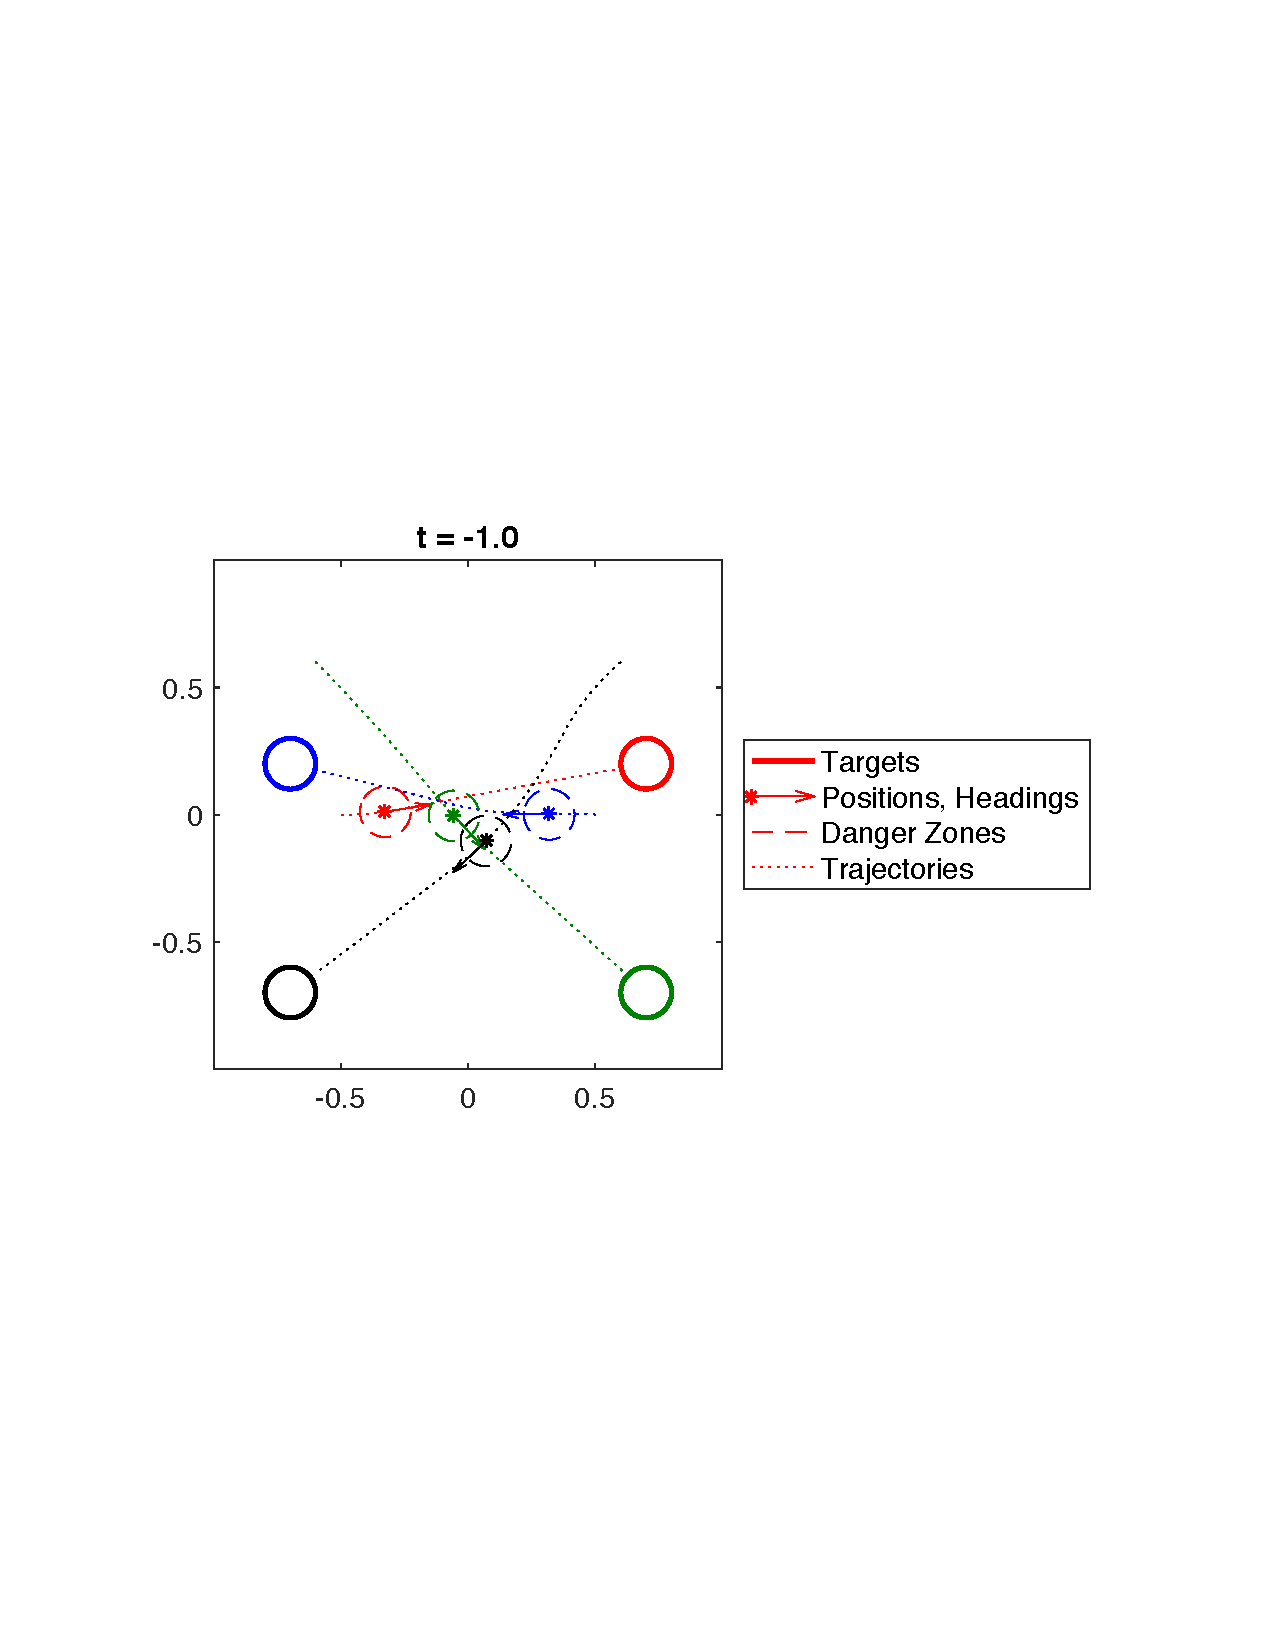
\includegraphics[width=0.8\columnwidth]{fig/cc_traj}
  \caption{Simulated trajectories in the centralized control method. Since the higher priority vehicles induce relatively small obstacles in this case, vehicles do not deviate much from a straight line trajectory towards their respective targets, and arrive at a dense configuration similar to that in Fig. \ref{fig:dubins_result}.}
  \label{fig:cc_traj}
\end{figure}

\begin{figure}
  \centering
  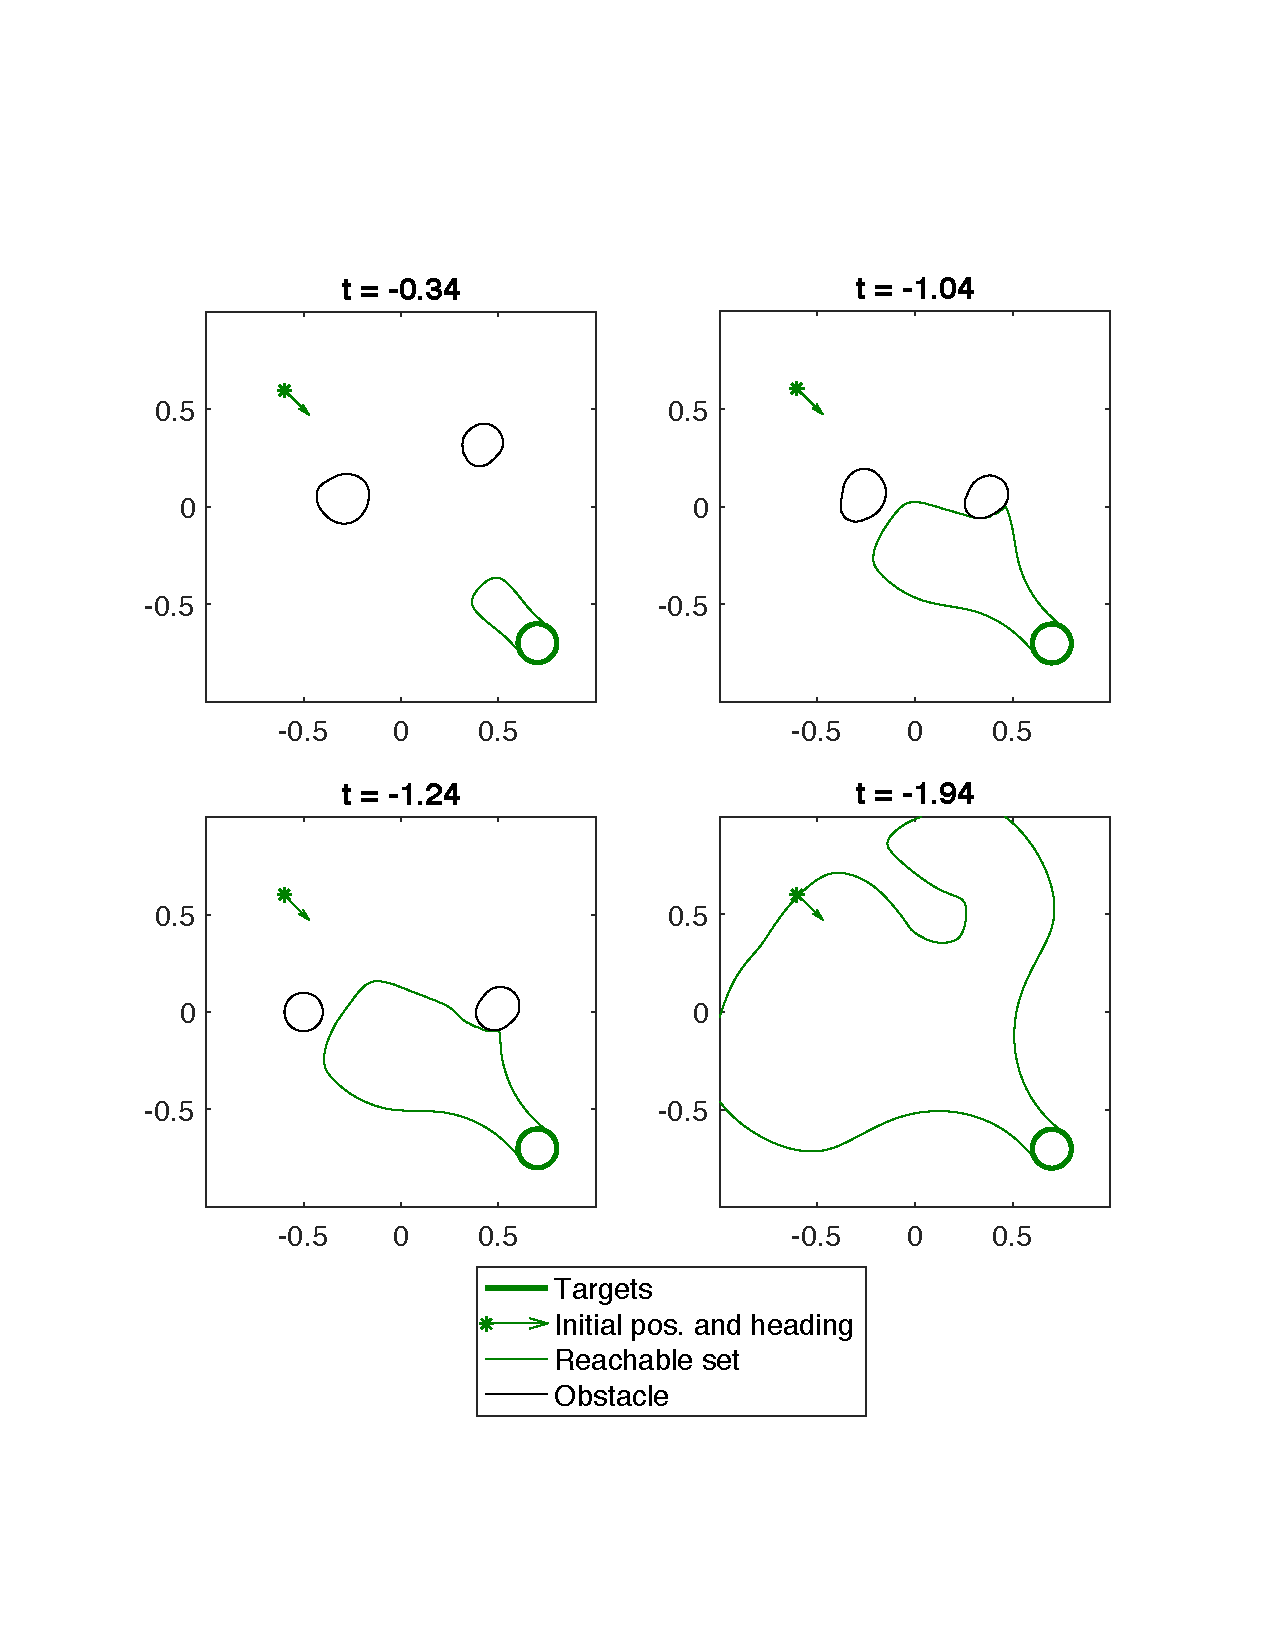
\includegraphics[width=0.9\columnwidth]{fig/cc_rs3}
  \caption{Evolution of the BRS and the obstacles induced by $\veh_1$ and $\veh_2$ for $\veh_3$ in the centralized control method. Since vehicles apply the optimal control at all times, the obstacle sizes are only slightly bigger than those in Fig. \ref{fig:dubins_reach_all} and \ref{fig:dubins_reach_3}.}
  \label{fig:cc_rs3}
\end{figure}